\documentclass{article}
\usepackage{booktabs}
\usepackage{graphicx}
\title{LZW inspired De-Duplication algorithm for variable size blocks}
\author{Justin}
\date{}
\begin{document}
   \maketitle
   \section{Introduction}
   The variable size defined in the title is a multiple of the smallest block size. So if the block size is 1 KB then the variable size blocks can be of 1, 2, 3 $\cdots$ KBs. In the project I would be utilizing 4 KB blocks(debatable). I haven't yet decided whether to put an upper limit on the block size, but I am just limiting my self to 32 KB, which is 8 block long ( highly unlikely to occur ). So the block sizes will vary as a multiple of 4, ie. 4, 8, 12, 16, $\cdots$ 32 KB. An empty dictionary is used, as pre-calculating the hashes for all the blocks and adding to dictionary would be expensive on time and space. The dictionary is used only during de-duplication, and is not utilized while retrieving the original data from the de-duplicated data.
   \section{Algorithm - De-Duplication}
   \begin{enumerate}  
   \item Start
   \item Initialize p (present) = false, size (number of matched blocks) = 0, i = 1
   \item Retrieve next (first during the first retrieval) block. ($B_i$)
   \item Compute hash of blocks $B_j, j \in [1,i]$  ($H_i$)
   \item Check if $H_i$ is present in the dictionary: if No goto step 7.
   \item If yes, set p = true, size = size + 1, i = i+1. goto step 3.
   \item If no, Add hash to dictionary.
   \item Check if p = false. if No goto step 10.
   \item If yes, retrieve next block, recompute hash, add to dictionary. Print block as it is, as its not a duplicate. Goto step 11.
   \item If no, print  (index of duplicate\_block, size), Set p = false, size = 0, i = 1, move read head one block back.
   \item Check if last block. If No goto step 3, else end.
\end{enumerate}  
   \begin{figure}
   \centering
    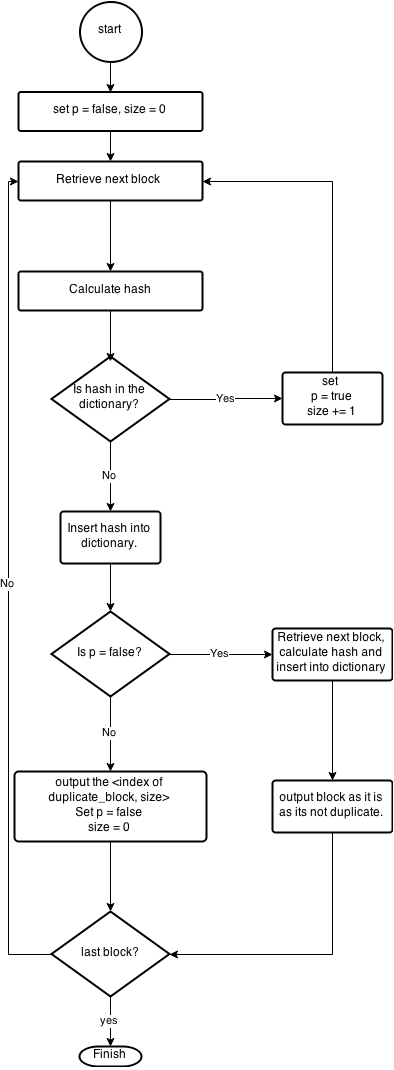
\includegraphics[scale=0.5]{dedupAlgo.png}
    \caption{LZW inspired variable block de duplication}
   \end{figure}
   
   \section{Re-duplication}
   \begin{enumerate}
   \item Start
   \item Read next/first entry of de-duplicated data.
   \item If data block: output as it is.
   \item Else if: index reference, then print blocks from the index till index+size.
   \item Last entry? if yes end, else goto step 2.
   \end{enumerate}
   \section{Example}
   Consider the blocks be "ABABCABBBCABCCC" where each alphabet represents a block of 4KB and the alphabet values can be considered as the hash value.\\
\\
   \begin{tabular}{|c|c|}
   \hline
   \textbf{Index}&\textbf{Value} \\
   \hline
   0 & A\\
   1 & B\\
   2 & A\\
   3 & B\\
   4 & C\\
   $\cdots$&$\cdots$\\
   \hline   
   \end{tabular}\\
  \\
   Input = "ABABCABBBCABCCC"
   \begin{table}[!th]
   \begin{tabular}{|c|c|c|}
   \hline
   \textbf{Sl. No.} & \textbf{Dictionary Value} & \textbf{Output Value} \\
   \hline
   1 & A & -\\
   2 & AB & A\\
   3 & B & -\\
   4 & BA & B\\
   5 & ABC & (0,2)\\
   6 & C & -\\
   7 & CA & C\\
   8 & ABB & (0,2)\\
   9 & BB & (1,1)\\
   10 & BC & (1,1)\\
   11 & CAB & (4,2)\\
   12 & BCC & (3,2)\\
   13 & CC & (4,1)\\
   14 & - & (4,1)\\
   \hline
   \end{tabular}
   \end{table}
   \newpage
   \subsection{Re Duplication}
   Input = "AB(0,2)C(0,2)(1,1)(1,1)(4,2)(3,2)(4,1)(4,1)"
   \begin{table}[!th]
   \begin{tabular}{|c|c|c|}
   \hline
   \textbf{Serial No.} & \textbf{Input Value} & \textbf{Output Value} \\
   \hline
   1 & A & A\\
   2 & B & B\\
   3 & (0,2) & AB (start at index 0, print 2 blocks)\\
   4 & C & C\\
   5 & (0,2) & AB\\
   6 & (1,1) & B\\
   7 & (1,1) & B\\
   8 & (4,2) & CA\\
   9 & (3,2) & BC\\
   10 & (4,1) & C\\
   11 & (4,1) & C\\
   \hline
   \end{tabular}
   \end{table}
\end{document}

